%\documentclass[]{openjournal}
\documentclass[manuscript, letterpaper]{aastex6}
\bibliographystyle{aasjournal}

\bibliographystyle{apj}
\usepackage{graphicx}
\usepackage[suffix=]{epstopdf}
\usepackage{natbib}
\usepackage{amsmath}
\usepackage{url}
\usepackage{xspace}


% from here: https://github.com/dfm/peerless/blob/master/document/ms.tex#L19-L69
% ----------------------------------- %
% start of AASTeX mods by DWH and DFM %
% ----------------------------------- %

\setlength{\voffset}{0in}
\setlength{\hoffset}{0in}
\setlength{\textwidth}{6in}
\setlength{\textheight}{9in}
\setlength{\headheight}{0ex}
\setlength{\headsep}{\baselinestretch\baselineskip} % this is 2 lines in ``manuscript''
\setlength{\footnotesep}{0in}
\setlength{\topmargin}{-\headsep}
\setlength{\oddsidemargin}{0.25in}
\setlength{\evensidemargin}{0.25in}

\linespread{0.54} % close to 10/13 spacing in ``manuscript''
\setlength{\parindent}{0.54\baselineskip}
\hypersetup{colorlinks = false}
\makeatletter % you know you are living your life wrong when you need to do this
\long\def\frontmatter@title@above{
\vspace*{-\headsep}\vspace*{\headheight}
\noindent\footnotesize
{\noindent\footnotesize\textsc{\@journalinfo}}\par
{\noindent\scriptsize Preprint typeset using \LaTeX\ style AASTeX6\\
With modifications by David W. Hogg and Daniel Foreman-Mackey
}\par\vspace*{-\baselineskip}\vspace*{0.625in}
}%
\makeatother

% Section spacing:
\makeatletter
\let\origsection\section
\renewcommand\section{\@ifstar{\starsection}{\nostarsection}}
\newcommand\nostarsection[1]{\sectionprelude\origsection{#1}}
\newcommand\starsection[1]{\sectionprelude\origsection*{#1}}
\newcommand\sectionprelude{\vspace{1em}}
\let\origsubsection\subsection
\renewcommand\subsection{\@ifstar{\starsubsection}{\nostarsubsection}}
\newcommand\nostarsubsection[1]{\subsectionprelude\origsubsection{#1}}
\newcommand\starsubsection[1]{\subsectionprelude\origsubsection*{#1}}
\newcommand\subsectionprelude{\vspace{1em}}
\makeatother

\widowpenalty=10000
\clubpenalty=10000

\sloppy\sloppypar

% ------------------ %
% end of AASTeX mods %
% ------------------ %


%    Make Scientific Notation
\providecommand{\e}[1]{\ensuremath{\times 10^{#1}}}

% make the word Kepler italicized
\newcommand{\Kepler}{\textsl{Kepler}\xspace}


\begin{document}
%%%%%%%%%%%%%%%%%%%%%%
\title{SETI in the Spatial-Temporal Domain}

\shorttitle{SETI in the Spatial-Temporal Domain}
\shortauthors{Davenport}

\author{
	James R. A. Davenport\altaffilmark{1,2}
	}

%\altaffiltext{1}{Corresponding author: James.Davenport@wwu.edu}
\altaffiltext{1}{Department of Physics \& Astronomy, Western Washington University, Bellingham, WA 98225}
\altaffiltext{2}{NSF Astronomy and Astrophysics Postdoctoral Fellow}
 

%%%%%%%%%%%%%%%%%%%%%%%%%%%%%%
\begin{abstract}
Traditional searches for extraterrestrial intelligence (SETI) focuses on temporal or multi-wavelength studies of single stars to detect transient or excess photon emission from artificial sources. However, the latest generation of synoptic time domain surveys enables a spatial-temporal SETI, where signals originate from resolved sources or multiple stars. Here I propose one such SETI approach, which utilizes exoplanet-like transit signals coordinated around multiple stars to indicate the presence of an interstellar civilization. Artificial planets would act as beacons, being placed in orbit around stars surrounding a home star system. The orbital period of each artificial satellite would be proportional to the distance from the beacon star to the home star system. If the orbital period versus beacon distance relationship was known, the exact location of the home system could be determined via triangulation (or trilateration) from a subset of the transit beacons. Current and future exoplanet surveys may be able to detect such spatially coordinated transits around nearby low-mass stars. Importantly, the spatial-temporal domain deserves increased attention from SETI researchers.
\end{abstract}


%%%%%%%%%%%%%%%%%%%%%%%%%%%%%%
\section{Introduction}

In the search for extraterrestrial intelligence (SETI), most approaches focus on direct detection of photons originating from transmission or waste energy. These searches occur over a range of wavelengths, and require extraterrestrials to produce sufficient radiation to be detected apart from their parent star. While this may be feasible at radio wavelengths, it is much more difficult in the optical regime where much of our time domain surveys operate. However,  it is more simple to block significant light from a star than to produce enough to out shine it, which has led to recent studies of time domain data for signatures of transiting artificial structures. 

Previous work has suggested looking for SETI signals from interstellar ``beacons''
\cite{benford2008}
However, most such work has been focused on using lasers or other means to out-shine a parent star, often observed using spectroscopy \cite{reines2002}. This is a very expensive way to stand out, and a slow way to find it, and so far has no success in discovering ET laser emission \cite{tellis2015}


optical seti
http://arxiv.org/abs/astro-ph/0506758

Instead, much cheaper to block light, rather than shine it.
\cite{arnold2005}
on the feasibility of transits for use in SETI detection, and 
\cite{arnold2005a}
on the impact of artificial structures on transits. also this work on that:
\cite{wright2016}.
recent data from \Kepler \citep{borucki2010}, has found weird transit-like signals
\cite{boyajian2015}, 
which some have considered as SETI candidates. However, follow-up observations have yet to yield any confirming signatures, and instead this looks like a YSO w/ comets maybe \citep{lisse2015}.

active and passive SETI in coordination (both temporal and spatial) with galactic events like supernovae 
\citep{lemarchand1994}

lighthouses
\citep{zuluaga2015}


\cite{arnold2005} note that objects could be placed at interesting spacing along the orbit to encode a pattern or simple message, demonstrating an intelligent origin. However, very little information can be effectively transmitted using eclipses, even with extreme precision in the recovery.


In this work we propose a new type of beacon system, which relies on ET transit signals from multiple stars to collectively ``point'' towards an ET civilization. This system has the advantage of being potentially detectable in the near future via exoplanet searches.




%%%%%%%%%%%%%%%%%%%%%%%%%%%%%%
\section{Example: Coordinated Transits as ET Beacons}
imagine a Type N civilization with the ability to both travel to nearby star systems, and to build large enough structures in orbit around other stars to produce a visible transit in our data.

give the detailed example i have thought up.

becons placed at distances


\begin{figure}[]
\centering
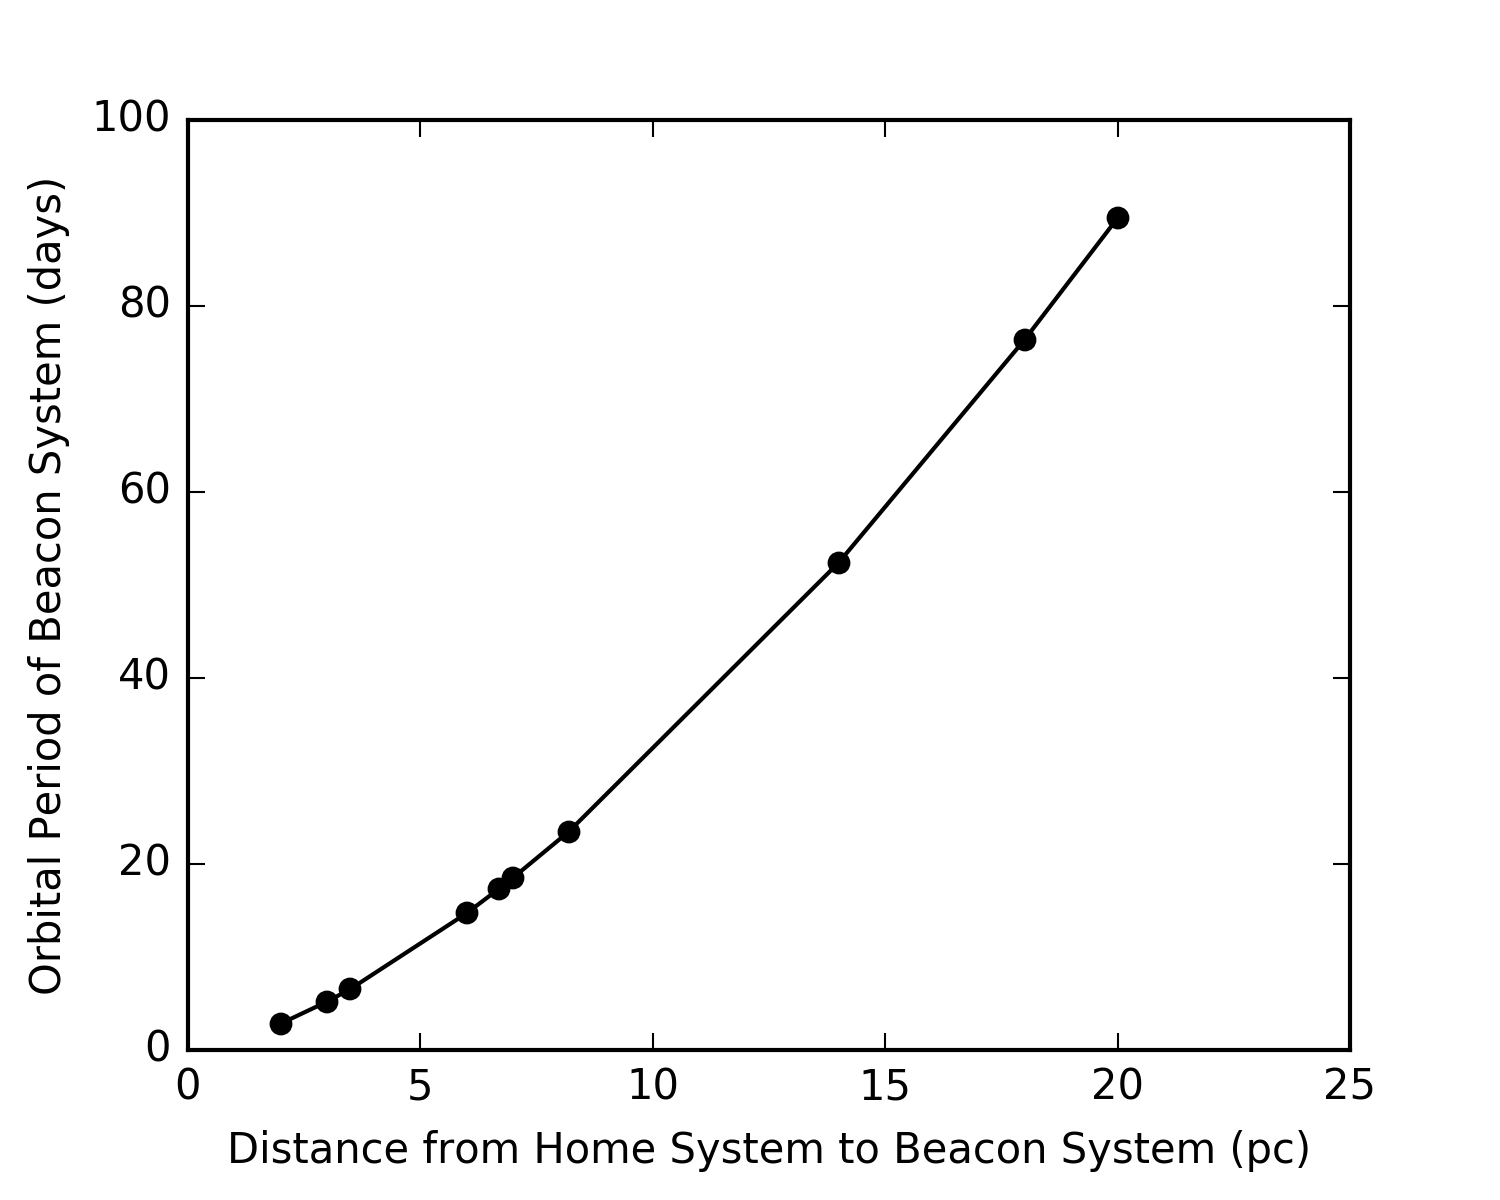
\includegraphics[width=3.5in]{../figures/dist_per.png}
\caption{schematic figure of the signal to detect in 1 dimension}
\label{fig:1d}
\end{figure}


for clarity, this is what the ideal signal might look like on the sky

\begin{figure}[]
\centering
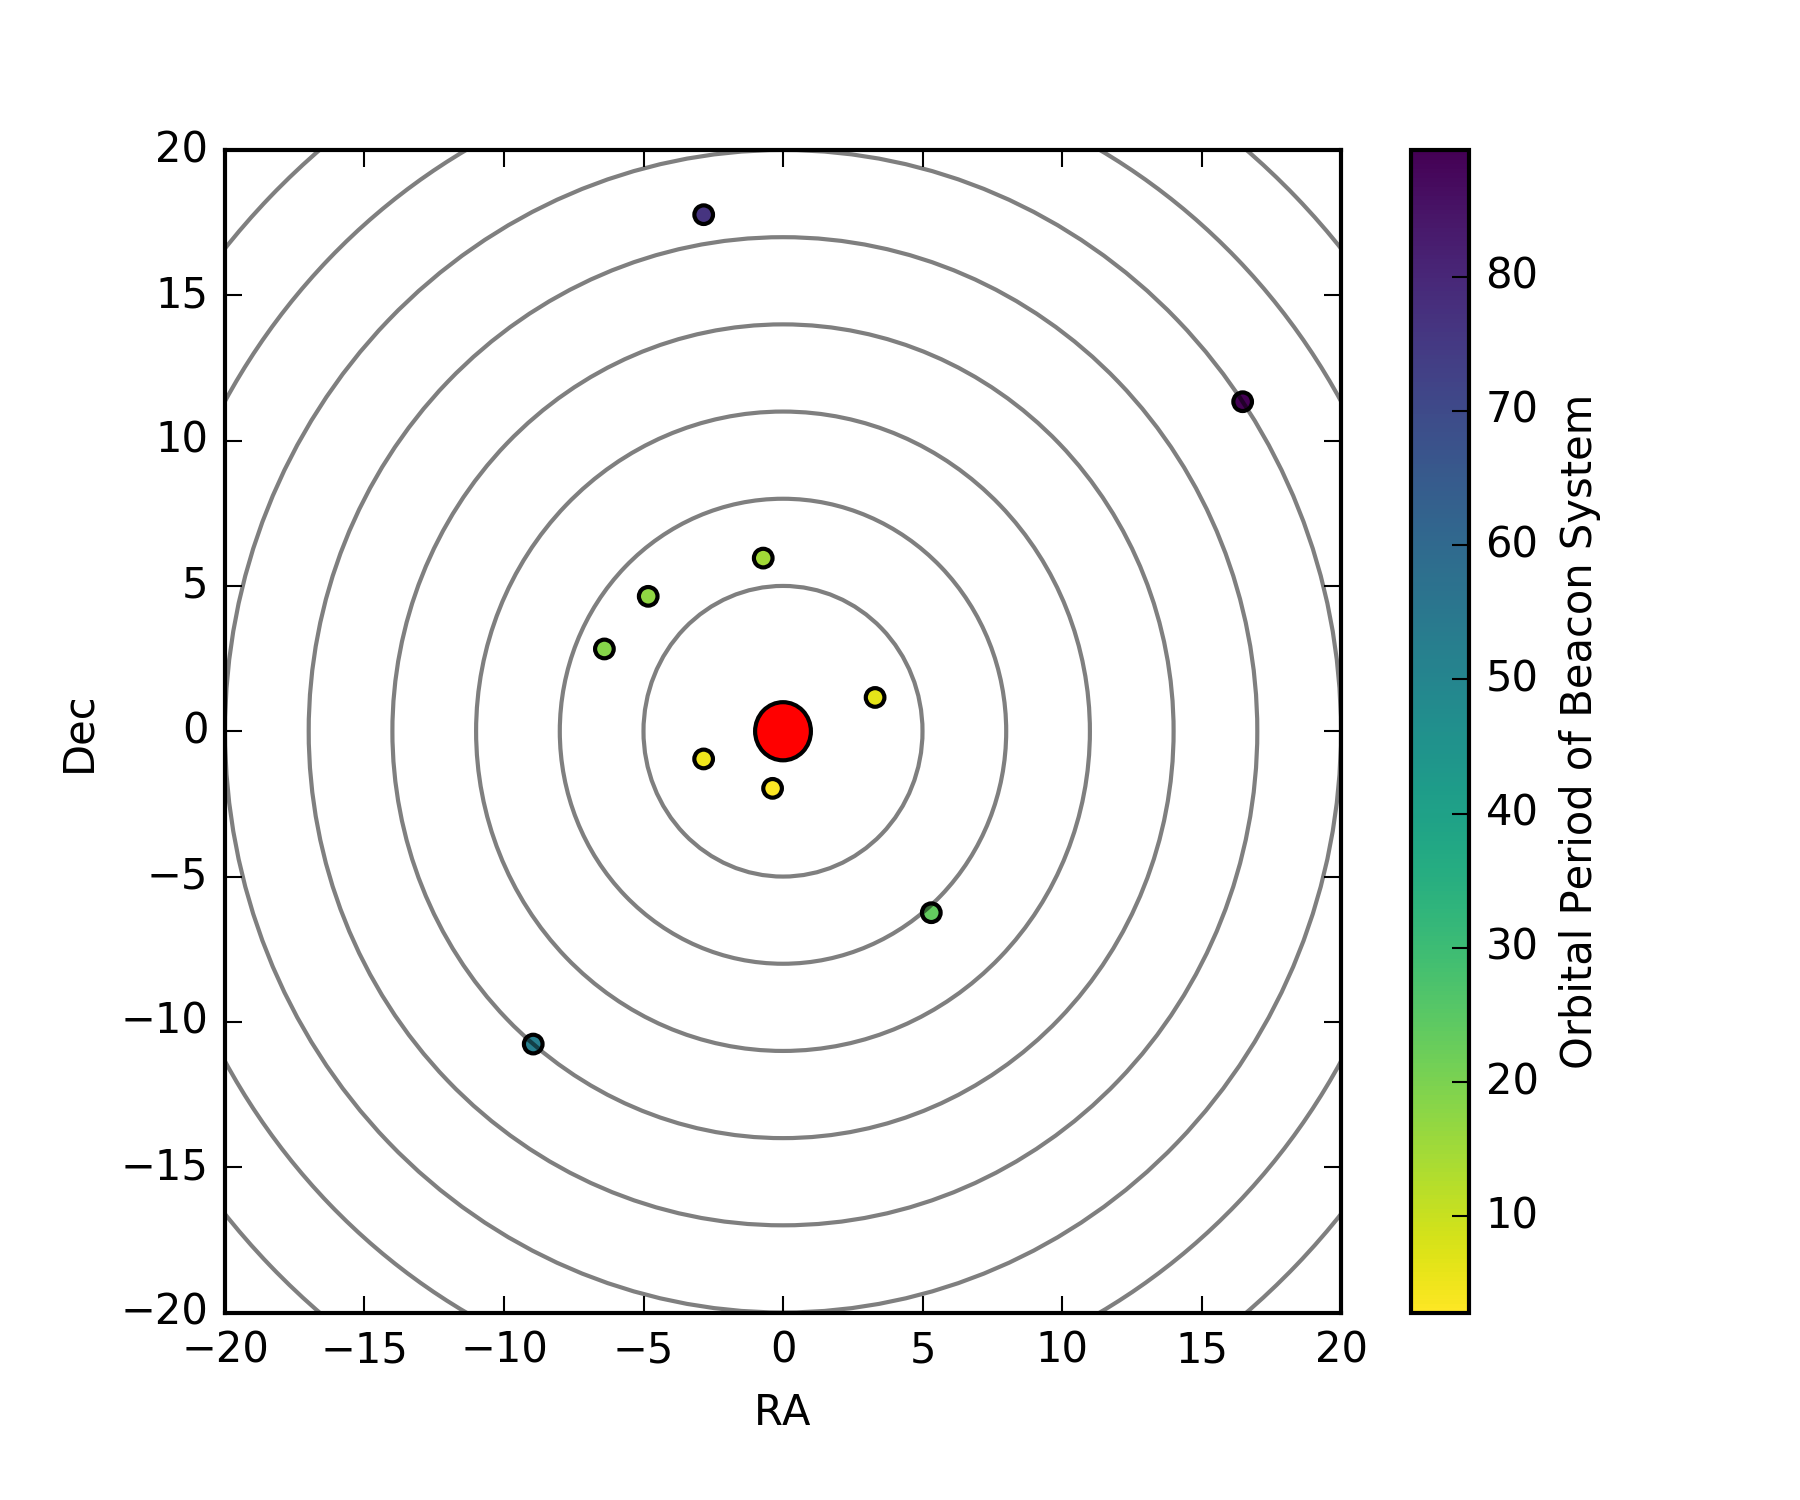
\includegraphics[width=3.5in]{../figures/sky_per.png}
\caption{schematic figure of the signal to detect in 2 dimensions. ra,dec in arbitrary units. red circle in middle is the home system}
\label{fig:2d}
\end{figure}


%and then what it might look like in 3d, projected in to 2d


%%%

this type of beacon network is advantageous because it points directly back towards their home. only a few systems actually need to be transiting from any given line of sight.

NOW THE FULL SIMULATION...
- computation to do: if had 100 beacons, each placed at random orbital alignment, in 3d sphere around home system.
- assume G stars, 
- odds of observing transit of a fixed sized object versus orbital distance... goes down. need that plot to figure out probability. 
- assume ET places beacons with uniform RADIAL density in 3d space out to some maximum distance (even \# of systems as function of radial distance) in bins of 10pc out to 100 pc (i.e. 10 beacons in each 10pc bin)
- orbital period is exact for each system, no bins of period
- do Monte Carlo sim with these parameters to figure out how many transiting systems we'd observe 

---- make the plot for one MC realization of RA,Dec.... open circles for systems with no observed transits, colored for transits


%%%%%%%%%%%%%%%%%%%%%%%%%%%%%%
\section{Prospects for Future Surveys}

to get accurate census you need a complete time domain survey at some transit depth sensitivity out to some orbital period. going off our simulation, TESS might work for very short period planets

TESS would be great for this in terms of spatial-temporal coverage. 

LSST very good for finding SETI signals of this geometric style, but not ideal for events requiring such dedicating monitoring


%%%%%%%%%%%%%%%%%%%%%%%%%%%%%%
\section{Discussion}
this kind of distributed network could be very efficient at broadcasting the presence of a civilization. dust clouds could create sufficient "transit" signals, while not affecting orbital dynamics


%%%%%%%%%%%%%%%%%
\acknowledgments
JRAD is supported by an NSF Astronomy and Astrophysics Postdoctoral Fellowship under award AST-1501418.

\bibliography{/Users/james/research/references}

\end{document}